% Spanish Cantilevers -- feature overview
% Build: latexmk -pdf spanish_cantilevers.tex   (or pdflatex twice)
\documentclass[11pt,a4paper]{article}

\usepackage[T1]{fontenc}
\usepackage[utf8]{inputenc}
\usepackage{lmodern}
\usepackage[english]{babel}
\usepackage[margin=2.2cm]{geometry}
\usepackage{graphicx}
\usepackage{caption}
\usepackage{subcaption}
\usepackage{booktabs}
\usepackage{tabularx}
\usepackage{xcolor}
\usepackage{enumitem}
\usepackage{float}
\usepackage[section]{placeins}
\usepackage[hidelinks]{hyperref}

\definecolor{spanishred}{RGB}{150,42,36}
\captionsetup{font=small,labelfont={bf,color=spanishred}}
\setlist{itemsep=2pt,topsep=4pt}
\graphicspath{{img/}}

% figures: fill text pages generously and stack figure-only pages from the top
\renewcommand{\topfraction}{0.9}
\renewcommand{\bottomfraction}{0.8}
\renewcommand{\textfraction}{0.07}
\renewcommand{\floatpagefraction}{0.7}
\makeatletter
\setlength{\@fptop}{0pt}
\setlength{\@fpsep}{12pt plus 1fil}
\setlength{\@fpbot}{0pt plus 1fil}
\makeatother

\newcommand{\photocredit}[1]{\par\vspace{1pt}{\scriptsize\color{gray}#1}}
\newcommand{\shot}[2][\linewidth]{\includegraphics[width=#1]{game/#2}}

\title{\color{spanishred}\textbf{Spanish Cantilevers}\\[4pt]
\large Spanish overhead line equipment\\for \emph{Create: Pantographs \& Wires}}
\author{Feature overview}
\date{Minecraft 1.20.1 (Forge) \quad$\cdot$\quad version 0.1.0 \quad$\cdot$\quad October 2026}

\begin{document}

\maketitle

\begin{figure}[H]
  \centering
  \shot{portada.png}
  \caption{A stretch of line built with the add-on: Spanish flat lattice masts, wide Spanish cantilevers in
  zigzag held by diagonal stays, and the overhead wire of \emph{Create: Pantographs \& Wires}.}
\end{figure}

\begin{center}
\small\itshape Developed by a railway enthusiast.
\end{center}

\newpage
\tableofcontents
\newpage

% ---------------------------------------------------------------------------
\section{Overview}

\textbf{Spanish Cantilevers} is an add-on for \emph{Create: Pantographs \& Wires} (PNW) that adds overhead
line equipment as it is built on the Spanish railway network:
the cantilevers (\emph{m\'ensulas}) of the conventional network, the masts that carry them, the rigid
overhead conductor rail used in tunnels and a Spanish-style pantograph.

The add-on does not replace any part of PNW. It plugs into PNW's wire system: its blocks are PNW wire
connectors, the catenary wire of PNW is strung onto them as usual, pantographs collect current from them in
the same way, and the masts share PNW's tags, so PNW blocks and Spanish blocks can be mixed freely on the
same line.

\paragraph{Contents of the add-on}
\begin{itemize}
  \item \textbf{Spanish Cantilever} -- a configurable cantilever modelled on the real one, with three
        zigzag positions, three insulator types, widths from 1.5 to 6.5 blocks, an optional support wire and,
        on wide cantilevers, a diagonal stay to the mast (Section~\ref{sec:cantilever}).
  \item \textbf{Spanish masts} -- flat lattice (straight and diagonal) and square lattice masts with four
        weathering stages and waxing (Section~\ref{sec:masts}).
  \item \textbf{Rigid catenary} -- an overhead conductor rail strung like a wire, which follows curves and
        can be joined to the flexible catenary (Section~\ref{sec:rigid}).
  \item \textbf{Spanish Tunnel Support} -- ceiling and wall supports for the rigid catenary in several
        variants, with an overall size setting that enlarges the support and its profile (Section~\ref{sec:tunnel}).
  \item \textbf{Spanish Pantograph} -- PNW's pantograph with the red frame typical of Spanish trains
        (Section~\ref{sec:pantograph}).
\end{itemize}

% ---------------------------------------------------------------------------
\section{Real-world reference}

On the Spanish conventional network the contact wire is usually held by \emph{cantilevers}: a steel tube
fixed to a lattice or H-beam mast, which rises in a short diagonal and then runs horizontally over the track.
The messenger wire rests on an insulator on top of the tube, and a registration arm hanging from the
cantilever pulls the contact wire alternately to each side of the track (\emph{zigzag}), so that the
pantograph strip wears evenly. A support wire (stay) often runs from the mast to the elbow of the tube.

\begin{figure}[htbp]
  \centering
  \begin{subfigure}[t]{0.49\linewidth}
    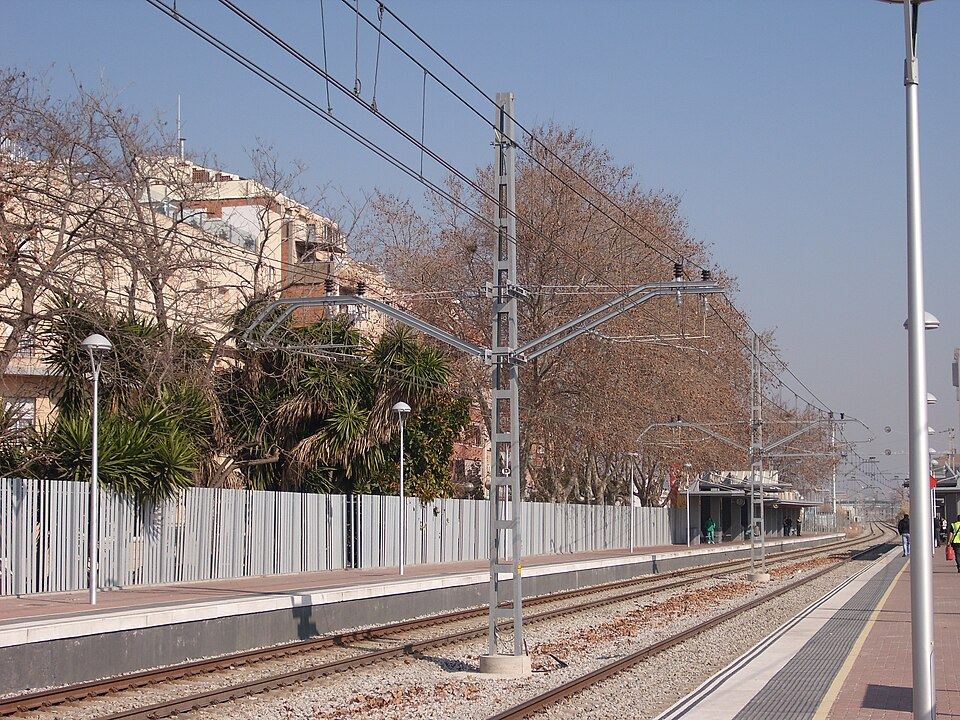
\includegraphics[width=\linewidth]{photos/sant_adria.jpg}
    \caption{Cantilevers on lattice masts, Sant Adri\`a de Bes\`os.}
    \photocredit{Adif -- Ineco, CC BY-SA 3.0, via Wikimedia Commons.}
  \end{subfigure}\hfill
  \begin{subfigure}[t]{0.49\linewidth}
    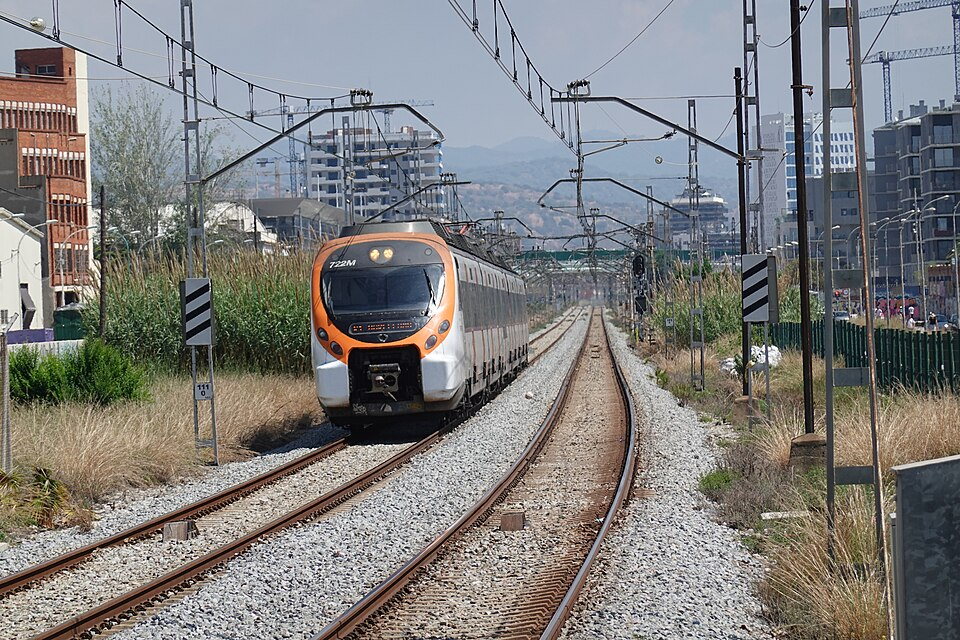
\includegraphics[width=\linewidth]{photos/sant_adria_rodalies.jpg}
    \caption{Commuter train under cantilevers on lattice masts, Sant Adri\`a de Bes\`os.}
    \photocredit{Smiley.toerist, CC BY-SA 4.0, via Wikimedia Commons.}
  \end{subfigure}
  \caption{Cantilevers of the Spanish conventional (Iberian gauge) network.}
\end{figure}

\begin{figure}[htbp]
  \centering
  \begin{subfigure}[t]{0.49\linewidth}
    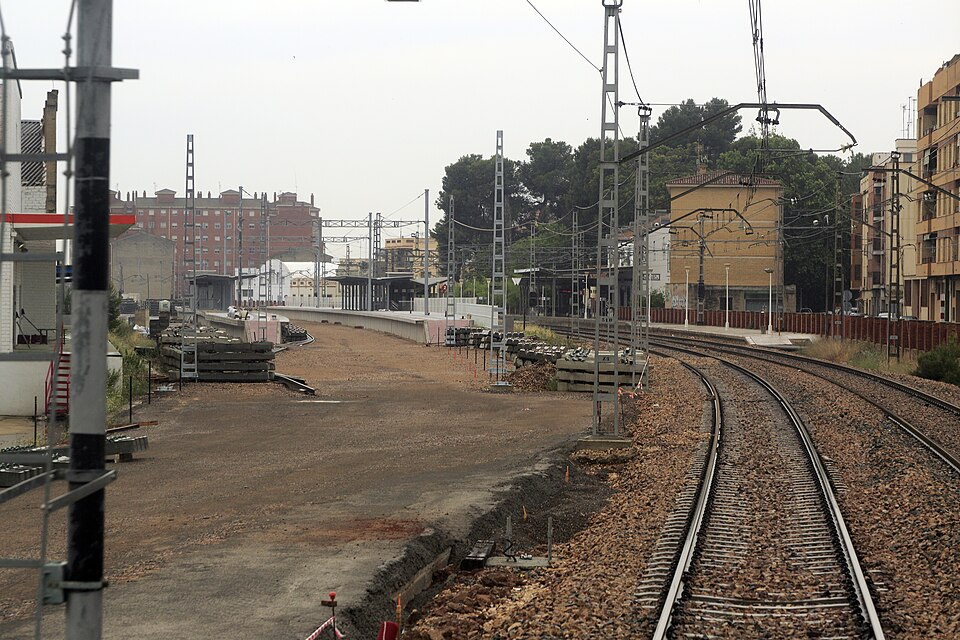
\includegraphics[width=\linewidth]{photos/nules.jpg}
    \caption{Conventional line with cantilevers on lattice masts, Nules (Valencia--Castell\'on).}
    \photocredit{Falk2, CC BY-SA 4.0, via Wikimedia Commons.}
  \end{subfigure}\hfill
  \begin{subfigure}[t]{0.49\linewidth}
    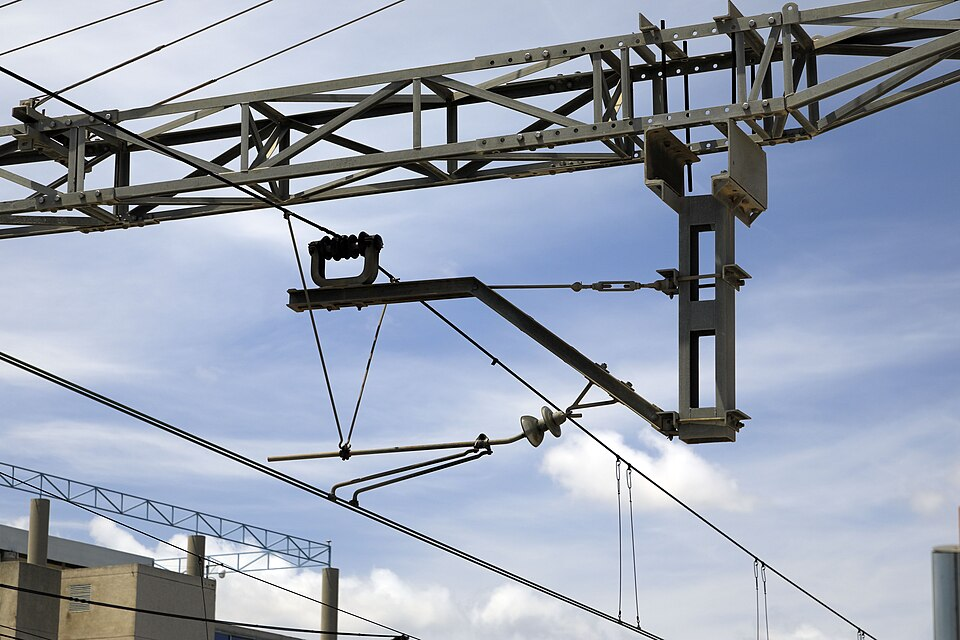
\includegraphics[width=\linewidth]{photos/valencia_registration_arm.jpg}
    \caption{Detail of a cantilever with its insulators and registration arm, Val\`encia Font de Sant Llu\'is.}
    \photocredit{Falk2, CC BY-SA 4.0, via Wikimedia Commons.}
  \end{subfigure}
  \caption{Conventional catenary in the Valencia area.}
\end{figure}

In tunnels and underground stations the flexible catenary is often replaced by a \emph{rigid catenary}:
an aluminium or steel profile that clamps the contact wire and hangs from short supports fixed to the
ceiling or to the tunnel wall. It needs very little height and almost no maintenance of tension.

\begin{figure}[htbp]
  \centering
  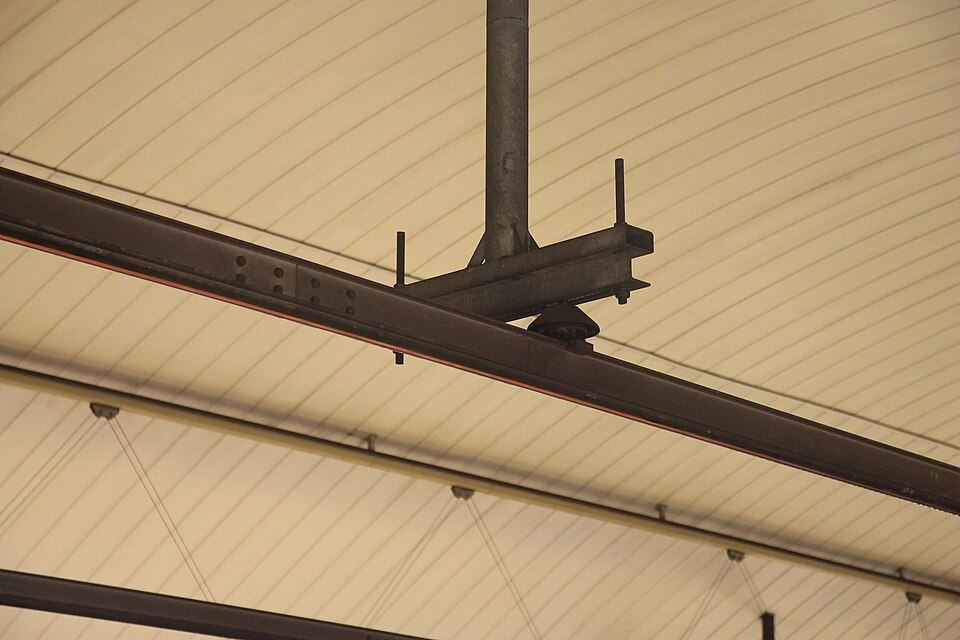
\includegraphics[width=0.7\linewidth]{photos/rigid_nuevos_ministerios.jpg}
  \caption{Rigid catenary and its ceiling supports, Nuevos Ministerios (Madrid Metro, Line 10).}
  \photocredit{Draceane, CC BY-SA 4.0, via Wikimedia Commons.}
\end{figure}

Many Spanish electric trains carry pantographs with a frame painted red, which is where the colour of the
Spanish Pantograph comes from.

\begin{figure}[htbp]
  \centering
  \begin{subfigure}[t]{0.49\linewidth}
    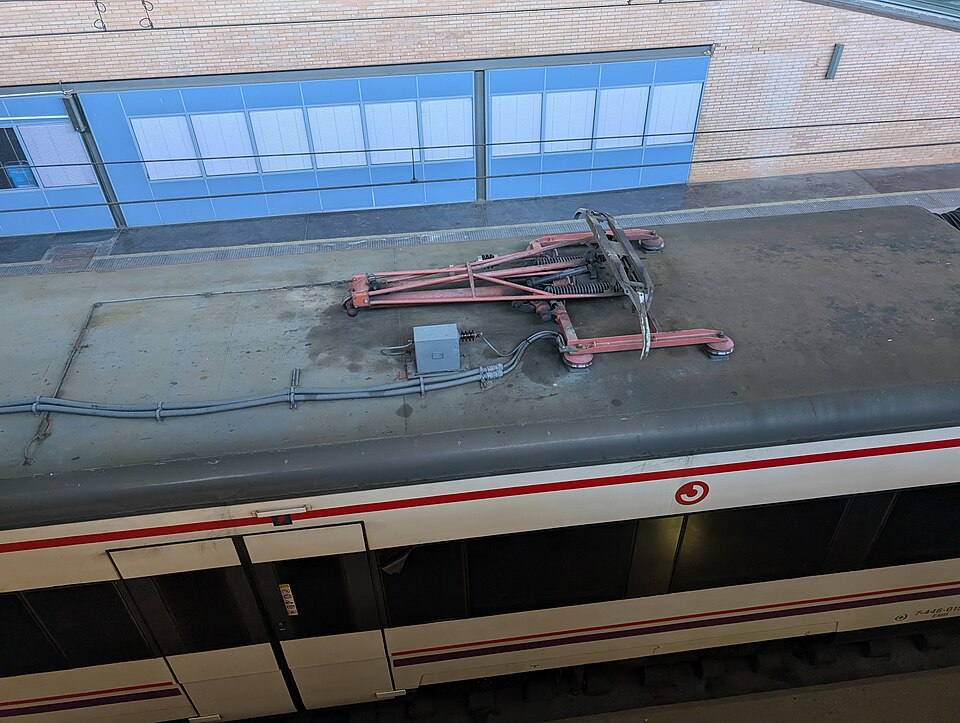
\includegraphics[width=\linewidth]{photos/pantograph_446.jpg}
    \caption{Pantograph on a Renfe Class 446 train, C\'ordoba.}
    \photocredit{Philip Mallis, CC BY-SA 4.0, via Wikimedia Commons.}
  \end{subfigure}\hfill
  \begin{subfigure}[t]{0.49\linewidth}
    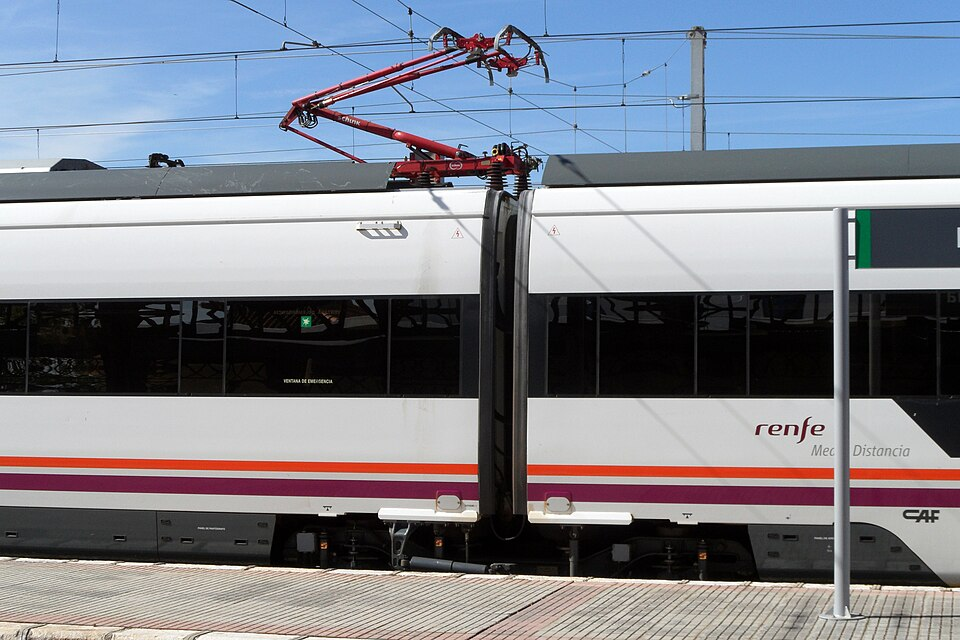
\includegraphics[width=\linewidth]{photos/pantograph_449.jpg}
    \caption{Pantograph on a Renfe Class 449 train.}
    \photocredit{Falk2, CC BY-SA 4.0, via Wikimedia Commons.}
  \end{subfigure}
  \caption{Red pantograph frames on Spanish trains.}
\end{figure}

% ---------------------------------------------------------------------------
\section{Spanish Cantilever}\label{sec:cantilever}

The Spanish Cantilever is placed on the side of a mast, exactly like PNW's cantilever, and accepts the PNW
catenary wire: the messenger wire is attached on top of the insulator and the contact wire at the tip of
the registration arm. All its parts are built from separate models (tube, perforated drop pieces,
registration arm, insulators, support wire) that are assembled and sized automatically from its settings,
so the cantilever always reaches exactly where the wires are.

\begin{figure}[htbp]
  \centering
  \shot{modos.png}
  \caption{The three zigzag positions of the contact wire: inner, middle and outer.}
\end{figure}

\subsection{Zigzag position}
\begin{itemize}
  \item \textbf{Inner} -- the contact wire is held towards the mast. The registration arm hangs from the
        diagonal or, for wide cantilevers, from an L-shaped strut below the horizontal tube.
  \item \textbf{Middle} -- the tube continues past the messenger insulator, drops at 45\textdegree{} into a
        perforated piece and a longer registration arm descends to the wire.
  \item \textbf{Outer} -- the tube drops into a diagonal and a vertical perforated piece, and the
        registration arm points back towards the mast.
\end{itemize}

\begin{figure}[htbp]
  \centering
  \begin{subfigure}[t]{0.325\linewidth}\shot{modo_interior.png}\caption{Inner.}\end{subfigure}\hfill
  \begin{subfigure}[t]{0.325\linewidth}\shot{modo_medio.png}\caption{Middle.}\end{subfigure}\hfill
  \begin{subfigure}[t]{0.325\linewidth}\shot{modo_exterior.png}\caption{Outer.}\end{subfigure}
  \caption{Side view of each zigzag position. The middle and outer positions use an arched registration
  arm with its own insulator.}
\end{figure}

\subsection{Insulator type and support wire}
The insulator that carries the messenger wire can be chosen among three types, and the support wire
(stay) between the mast and the elbow of the tube can be added or removed. Every insulator type works with
every zigzag position: the nine combinations are shown below.

\begin{itemize}
  \item \textbf{Horizontal support} -- the messenger rests on top of a horizontal insulator.
  \item \textbf{Horizontal hanging support} -- the insulator hangs below the tube and the messenger passes
        through it (shown without support wire).
  \item \textbf{Vertical support} -- a vertical insulator on top of the tube.
\end{itemize}

\begin{figure}[htbp]
  \centering
  \newcommand{\var}[2]{\begin{subfigure}[t]{0.325\linewidth}\shot{variante_#1.png}\caption{#2}\end{subfigure}}
  \var{tipo1_interior}{Horizontal support, inner.}\hfill
  \var{tipo1_medio}{Horizontal support, middle.}\hfill
  \var{tipo1_exterior}{Horizontal support, outer.}\\[4pt]
  \var{tipo2_interior}{Hanging support, inner.}\hfill
  \var{tipo2_medio}{Hanging support, middle.}\hfill
  \var{tipo2_exterior}{Hanging support, outer.}\\[4pt]
  \var{tipo3_interior}{Vertical support, inner.}\hfill
  \var{tipo3_medio}{Vertical support, middle.}\hfill
  \var{tipo3_exterior}{Vertical support, outer.}
  \caption{All nine combinations of insulator type (rows) and zigzag position (columns).}
\end{figure}

\subsection{Width}
The width is the distance from the mast to the track axis, from 1.5 to 6.5 blocks in one-block steps, as
with PNW's cantilever. The tube, the diagonal and the registration arm are sized automatically for each
width, so the messenger always sits above the track and the contact wire at its zigzag position.

\begin{figure}[htbp]
  \centering
  \shot{anchuras.png}
  \caption{The six widths, from 1.5 (left) to 6.5 blocks (right), on Spanish square lattice masts.}
\end{figure}

\subsection{Diagonal stay}
Wide cantilevers (width 3 or more) can be hung from the mast with a \emph{diagonal stay}. With PNW's wire
coil set to \emph{Support Wire}, click the cantilever and then a block of the mast between 2 and 5 blocks
above it (or the other way round). The stay is a single straight wire that enters the horizontal tube just
before the messenger insulator and the face of the mast that looks towards the cantilever, so it looks
fastened to the steel at both ends.

\begin{itemize}
  \item The attachment point on the tube moves outwards with the width, so the stay always holds the far end
        of the cantilever.
  \item The height on the mast is chosen by the block that is clicked (2 to 5 blocks above the cantilever),
        which gives different triangles.
  \item If the cantilever is reconfigured the stay follows it; if it becomes narrower than 3 blocks the stay
        is removed. Breaking the cantilever or that mast block returns the wire to the coil.
\end{itemize}

\begin{figure}[htbp]
  \centering
  \shot{tirante_anchuras.png}
  \caption{Diagonal stays on cantilevers of width 3.5, 4.5, 5.5 and 6.5, all to a mast block 3 blocks
  higher: the attachment on the tube moves outwards with the width.}
\end{figure}

\begin{figure}[htbp]
  \centering
  \shot{tirante_alturas.png}
  \caption{The same cantilever (width 4.5) with the stay 2, 3, 4 and 5 blocks up the mast.}
\end{figure}

\begin{figure}[htbp]
  \centering
  \begin{subfigure}[t]{0.49\linewidth}\shot{tirante_metido.png}\caption{The stay enters the horizontal tube before
  the messenger insulator.}\end{subfigure}\hfill
  \begin{subfigure}[t]{0.49\linewidth}\shot{tirante_poste.png}\caption{The stay enters the face of the mast.}\end{subfigure}
  \caption{Both ends of the diagonal stay.}
\end{figure}

\subsection{Settings window}
Right-clicking with the cantilever item in hand (or with an empty hand on a placed cantilever) opens a
settings window in the same style as PNW's, with a live 3D preview.

\begin{figure}[htbp]
  \centering
  \shot[0.75\linewidth]{ventana_mensula.png}
  \caption{Settings window of the Spanish Cantilever.}
\end{figure}

\begin{center}
\begin{tabularx}{\linewidth}{@{}lX@{}}
\toprule
\textbf{Setting} & \textbf{Effect} \\
\midrule
Width & Reach of the cantilever from the mast to the track axis, from 1.5 to 6.5 blocks. \\
Insulator type & Horizontal support, horizontal hanging support or vertical support. \\
Contact wire & Zigzag position: inner, middle or outer. \\
Support wire & With or without the stay between mast and tube. \\
Supporter height & Drop of the diagonal of the tube (advanced). \\
Catenary height & Height of the contact wire below the block (advanced). \\
Y offset & Lowers the whole cantilever (advanced). \\
Set default config & Stores the current settings as the default for new, unconfigured items. \\
\bottomrule
\end{tabularx}
\end{center}

Without advanced options the heights follow fixed proportions, as PNW does with its own cantilever.
Changing the settings of a cantilever that already has wires attached moves the wires (and the diagonal
stay) with it.

\subsection{Placement}
\begin{itemize}
  \item Attaches to PNW masts, Spanish masts, concrete pillars and any other block that PNW's cantilever
        accepts, in the same 16 directions as PNW blocks (including 45\textdegree{} on diagonal masts).
  \item The mounting plate adapts to the thickness of the mast and widens on thick masts or full blocks
        without deforming its bolts.
  \item The item stacks up to 64.
\end{itemize}

\begin{figure}[htbp]
  \centering
  \shot{portada_cerca.png}
  \caption{An outer cantilever strung with PNW catenary wire (messenger, contact wire and droppers), with its
  support wire and diagonal stay.}
\end{figure}

% ---------------------------------------------------------------------------
\section{Spanish masts}\label{sec:masts}

Three mast families with a Spanish finish: \emph{Spanish Flat Lattice Mast}, \emph{Spanish Flat
Diagonal Lattice Mast} and \emph{Spanish Lattice Mast} (square section). They reuse PNW's mast behaviour:
\begin{itemize}
  \item four weathering stages (new, exposed, weathered, oxidized) that progress over time;
  \item waxing with honeycomb and wax removal with an axe, as with PNW masts;
  \item the same connection tags as PNW masts, so both PNW's cantilevers and Spanish Cantilevers attach to
        them, and the flat mast can be switched between its straight and diagonal versions by crafting.
\end{itemize}

\begin{figure}[htbp]
  \centering
  \shot{postes.png}
  \caption{The three Spanish masts -- flat lattice, flat diagonal lattice and square lattice -- each in its
  four weathering stages: new, exposed, weathered and oxidized.}
\end{figure}

% ---------------------------------------------------------------------------
\section{Rigid catenary}\label{sec:rigid}

The \emph{Rigid Catenary Profile Bundle} is used like PNW's wire coil: click a support, then the next one,
and a rigid profile is laid between them. For PNW it is one more wire of the catenary network, so
pantographs collect current from it.

\begin{itemize}
  \item A bundle holds 200 metres of profile and is consumed by length; a bar shows what is left.
  \item Where two spans meet at a support with a gentle angle, the profile bends smoothly through the
        support instead of making a sharp corner.
  \item Breaking a span returns its metres to the bundles in the player's inventory; whatever does not fit is
        dropped as a single bundle.
\end{itemize}

\begin{figure}[htbp]
  \centering
  \shot{tunel_dentro.png}
  \caption{Rigid catenary through a tunnel, with ceiling supports alternating their clamp position to make
  the zigzag.}
\end{figure}

\begin{figure}[htbp]
  \centering
  \shot[0.8\linewidth]{curva.png}
  \caption{The profile following a curve: between supports it is laid in short straight pieces that bend
  smoothly through each clamp.}
\end{figure}

\subsection{Transition from flexible to rigid catenary}
PNW's catenary wire can be strung from a cantilever to a tunnel support. The contact wire enters the clamp of
the rigid profile and the messenger wire descends to an anchoring point just above it; at the transition
support the end of the profile turns towards the incoming contact wire so that the pantograph passes smoothly.
With default settings, a tunnel support placed under a ceiling at the height of a cantilever keeps the contact
wire level across the transition.

\begin{figure}[htbp]
  \centering
  \begin{subfigure}[t]{0.49\linewidth}\shot{tunel_boca.png}\caption{The flexible catenary entering the tunnel
  mouth.}\end{subfigure}\hfill
  \begin{subfigure}[t]{0.49\linewidth}\shot{transicion.png}\caption{Seen from inside: the rigid profile ends at the
  first support and the contact wire and messenger continue to the cantilever outside.}\end{subfigure}
  \caption{Transition between flexible and rigid catenary.}
\end{figure}

% ---------------------------------------------------------------------------
\section{Spanish Tunnel Support}\label{sec:tunnel}

A single block covers every support of the rigid catenary. It is configured from one settings window and
comes in two versions:

\begin{itemize}
  \item \textbf{Ceiling} -- hangs from the block above on a rod. Two sizes (normal and large, with
        cross-members spanning the whole block) and three clamp positions (left, centre, right) to build the
        zigzag. Its height can be increased in quarter-block steps; the rod stretches accordingly.
  \item \textbf{Wall} -- a horizontal insulated arm fixed to a wall, to the side of a PNW mast or to a
        concrete pillar, placed like a cantilever in 16 directions. Two arm lengths (short and long). Its height
        can be moved up or down within the block in half-pixel steps, starting from the centre.
\end{itemize}

The version is chosen automatically when placing: clicking the side of a wall or pillar places the wall
version, clicking the underside of a ceiling places the ceiling version.

\begin{figure}[htbp]
  \centering
  \newcommand{\sop}[2]{\begin{subfigure}[t]{0.325\linewidth}\shot{soporte_#1.png}\caption{#2}\end{subfigure}}
  \sop{normal_0}{Normal, left clamp.}\hfill
  \sop{normal_1}{Normal, centre clamp.}\hfill
  \sop{normal_2}{Normal, right clamp.}\\[4pt]
  \sop{grande_0}{Large, left clamp.}\hfill
  \sop{grande_1}{Large, centre clamp.}\hfill
  \sop{grande_2}{Large, right clamp.}
  \caption{Ceiling supports: both sizes with the three clamp positions, each with its rigid profile.}
\end{figure}

\begin{figure}[htbp]
  \centering
  \begin{subfigure}[t]{0.49\linewidth}\shot{vitrina_techo.png}\caption{Normal ceiling supports.}\end{subfigure}\hfill
  \begin{subfigure}[t]{0.49\linewidth}\shot{vitrina_grande.png}\caption{Large ceiling supports.}\end{subfigure}
  \caption{The three clamp positions side by side: left, centre and right.}
\end{figure}

\begin{figure}[htbp]
  \centering
  \begin{subfigure}[t]{0.49\linewidth}\shot{pared_corto.png}\caption{Short wall arm.}\end{subfigure}\hfill
  \begin{subfigure}[t]{0.49\linewidth}\shot{pared_largo.png}\caption{Long wall arm.}\end{subfigure}
  \caption{Wall version.}
\end{figure}

\subsection{Overall size}
The \emph{Overall size} setting (100\,\%, 125\,\% or 150\,\%) makes the whole set larger: the support and
the rigid profile strung from it. The ceiling version grows around its clamp, so the contact wire stays at the
same height and the rod still reaches the ceiling; the wall version grows from the wall, so its arm becomes
longer. Each span of profile takes the size of the support where it was started (the first click); supports of
different sizes can be joined on the same line.

\begin{figure}[htbp]
  \centering
  \newcommand{\esc}[2]{\begin{subfigure}[t]{0.325\linewidth}\shot{soporte_escala_#1.png}\caption{#2}\end{subfigure}}
  \esc{0}{100\,\%.}\hfill
  \esc{1}{125\,\%.}\hfill
  \esc{2}{150\,\%.}
  \caption{The normal ceiling support at the three overall sizes, with the profile at the same size.}
\end{figure}

\begin{figure}[htbp]
  \centering
  \shot[0.8\linewidth]{vitrina_escala.png}
  \caption{The three overall sizes side by side.}
\end{figure}

\subsection{Settings window}
\begin{center}
\begin{tabularx}{\linewidth}{@{}lX@{}}
\toprule
\textbf{Setting} & \textbf{Effect} \\
\midrule
Version & Ceiling or wall (also chosen automatically by the face that is clicked). \\
Size & Normal or large (ceiling); short or long arm (wall). \\
Clamp & Left, centre or right (ceiling only), to build the zigzag. \\
Height & Ceiling: how much longer the rod is. Wall: up or down from the centre of the block. \\
Overall size & 100\,\%, 125\,\% or 150\,\% for the support and the profile strung from it. \\
Set default config & Stores the current settings as the default for new, unconfigured items. \\
\bottomrule
\end{tabularx}
\end{center}

As with the cantilever, the window opens with the item in hand (and the settings are kept in the item) or with
an empty hand on a placed support; the wires already strung move with it.

\begin{figure}[htbp]
  \centering
  \begin{subfigure}[t]{0.49\linewidth}\shot{ventana_tunel.png}\caption{Ceiling version at 150\,\%, with the
  ceiling block shown for reference.}\end{subfigure}\hfill
  \begin{subfigure}[t]{0.49\linewidth}\shot{objeto_tunel.png}\caption{Wall version at 150\,\%, with the wall
  block shown for reference.}\end{subfigure}
  \caption{Settings window of the tunnel support.}
\end{figure}

% ---------------------------------------------------------------------------
\section{Spanish Pantograph}\label{sec:pantograph}

The Spanish Pantograph is PNW's pantograph with its frame painted red, as on many Spanish trains. It keeps
the model, animation and behaviour of the original: it can be raised and lowered, it collects current from
both the flexible and the rigid catenary, and it works on Create trains and contraptions. Insulators and the
contact strip keep their original colours.

\begin{figure}[htbp]
  \centering
  \shot[0.85\linewidth]{pantografos.png}
  \caption{PNW pantograph (left) and Spanish Pantograph (right).}
\end{figure}

% ---------------------------------------------------------------------------
\section{Items and crafting}

\begin{center}
\renewcommand{\arraystretch}{1.3}
\begin{tabularx}{\linewidth}{@{}m{1.4cm}lX@{}}
\toprule
& \textbf{Item} & \textbf{Recipe} \\
\midrule

\includegraphics[width=1cm]{items/spanish_steel.png} & Spanish Steel & Iron ingot and black dye (shapeless). Base
material of the add-on. \\
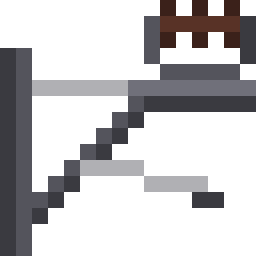
\includegraphics[width=1cm]{items/cantilever.png} & Spanish Cantilever & Create sequenced assembly from a PNW iron
rod bundle: two loops of deploying Spanish Steel, deploying a brown insulator and pressing. \\
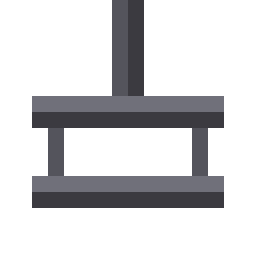
\includegraphics[width=1cm]{items/tunnel_support.png} & Spanish Tunnel Support & Two Spanish Steel above a brown
insulator; makes two. \\

\includegraphics[width=1cm]{items/rigid_profile.png} & Rigid Catenary Profile Bundle & Six Spanish Steel. \\
& Spanish masts & PNW iron strips with Spanish Steel (and iron rods for the square mast); six per craft. \\
& Spanish Pantograph & PNW pantograph and red dye (shapeless). \\
\bottomrule
\end{tabularx}
\end{center}

All recipes are visible in recipe viewers such as JEI, including the Create sequenced assembly.

% ---------------------------------------------------------------------------
\section{Technical summary}

\begin{center}
\begin{tabularx}{\linewidth}{@{}lX@{}}
\toprule
Minecraft & 1.20.1, Forge 47 \\
Required mods & Create: Pantographs \& Wires (1.20.1-beta-0.2.3-C6), Create 6.0.8, DragonLib, GeckoLib \\
License & GPL-3.0, the same as Pantographs \& Wires \\
Languages & English, Spanish, Catalan, German \\
Mod id & \texttt{spanishcantilevers} \\
\bottomrule
\end{tabularx}
\end{center}

\paragraph{Integration with Pantographs \& Wires}
The add-on relies only on PNW's public building blocks: wire connectors, wire types registered in PNW's wire
registry and catenary graph, PNW's mast classes and tags, its pantograph and its GUI widgets. Its own content
(models, textures, translations and code) is self-contained, so it can be distributed as a separate add-on that
requires PNW, or merged into PNW as a set of additional blocks.

\paragraph{Credits}
\emph{Create: Pantographs \& Wires} by MrJulsen, on which this add-on is built, and \emph{Create} by the Create
team. Photographs from Wikimedia Commons, credited under each image and listed below.

\begin{footnotesize}
\begin{itemize}
  \item \emph{Catenaria Sant Adrià (Adif)} -- Adif -- Ineco, CC BY-SA 3.0.
        \url{https://commons.wikimedia.org/wiki/File:Catenaria_Sant_Adri%C3%A0_(Adif).jpg}
  \item \emph{Sant Adrià de Besòs station 2023 2} -- Smiley.toerist, CC BY-SA 4.0.
        \url{https://commons.wikimedia.org/wiki/File:Sant_Adri%C3%A0_de_Bes%C3%B2s_station_2023_2.jpg}
  \item \emph{J23 477 Bf Nules-La Villavieja} -- Falk2, CC BY-SA 4.0.
        \url{https://commons.wikimedia.org/wiki/File:J23_477_Bf_Nules-La_Villavieja.jpg}
  \item \emph{L04 380 Bf Valencia Fuente San Luis, Fahrleitungsstützpunkt} -- Falk2, CC BY-SA 4.0.
        \url{https://commons.wikimedia.org/wiki/File:L04_380_Bf_Valencia_Fuente_San_Luis,_Fahrleitungsst%C3%BCtzpunkt.jpg}
  \item \emph{Nuevos Ministerios L10 catenaria rígida} -- Draceane, CC BY-SA 4.0.
        \url{https://commons.wikimedia.org/wiki/File:Nuevos_Ministerios_L10_catenaria_rigida.jpg}
  \item \emph{Pantograph on top of Renfe Class 446 train at Córdoba} -- Philip Mallis, CC BY-SA 4.0.
        \url{https://commons.wikimedia.org/wiki/File:Pantograph_on_top_of_Renfe_Class_446_train_at_C%C3%B3rdoba_Julio_Anguita_Railway_Station_in_C%C3%B3rdoba,_Spain_(55066435535).jpg}
  \item \emph{S01 882 Stromabnehmer BR 449} -- Falk2, CC BY-SA 4.0.
        \url{https://commons.wikimedia.org/wiki/File:S01_882_Stromabnehmer_BR_449.jpg}
\end{itemize}
\end{footnotesize}

% ---------------------------------------------------------------------------
\section*{Changelog}
10 October 2026:
  \begin{itemize}
    \item \textbf{Renamed} from \emph{Iberian Cantilevers} to \emph{Spanish Cantilevers} (mod id
          \texttt{spanishcantilevers}): Portugal's conventional network uses a different cantilever design, so
          the add-on now refers only to Spanish equipment. Blocks and items were renamed accordingly
          (\emph{Spanish Cantilever}, \emph{Spanish masts}, \emph{Spanish Steel}, \emph{Spanish Pantograph}).
  \end{itemize}
8 October 2026:
  \begin{itemize}
    \item \textbf{New:} diagonal stay for cantilevers of width 3 or more, strung with PNW's wire coil in
          \emph{Support Wire} mode from the horizontal tube to a mast block 2 to 5 blocks higher. It is a single
          wire that enters the tube and the mast, its attachment moves outwards with the width, it follows the
          cantilever when it is reconfigured and it returns its wire when broken.
    \item \textbf{New:} \emph{Overall size} of the tunnel support (100\,\%, 125\,\%, 150\,\%), which enlarges the
          support and the rigid profile strung from it; sizes can be mixed on the same line.
  \end{itemize}


\end{document}
